
\documentclass[11pt]{article}
\usepackage{cs65f10}
\usepackage{times}
\usepackage{latexsym}
\usepackage{graphics}
\usepackage{smiley}
\setlength\titlebox{6.5cm}    % Expanding the titlebox
\title{Analyzing the Relationship Between Tweets, Box-Office Performance, and Stocks}

% Alter some LaTeX defaults for better treatment of figures:
    % See p.105 of "TeX Unbound" for suggested values.
    % See pp. 199-200 of Lamport's "LaTeX" book for details.
    %   General parameters, for ALL pages:
    \renewcommand{\topfraction}{0.9}	% max fraction of floats at top
    \renewcommand{\bottomfraction}{0.8}	% max fraction of floats at bottom
    %   Parameters for TEXT pages (not float pages):
    \setcounter{topnumber}{2}
    \setcounter{bottomnumber}{2}
    \setcounter{totalnumber}{4}     % 2 may work better
    \setcounter{dbltopnumber}{2}    % for 2-column pages
    \renewcommand{\dbltopfraction}{0.9}	% fit big float above 2-col. text
    \renewcommand{\textfraction}{0.07}	% allow minimal text w. figs
    %   Parameters for FLOAT pages (not text pages):
    \renewcommand{\floatpagefraction}{0.7}	% require fuller float pages
	% N.B.: floatpagefraction MUST be less than topfraction !!
    \renewcommand{\dblfloatpagefraction}{0.7}	% require fuller float pages

	% remember to use [htp] or [htpb] for placement

\author{Catie Meador\\
  Swarthmore College\\
  500 College Ave\\
  Swarthmore PA 19081\\
  {\tt cmeador1@cs.swarthmore.edu}  
  \And
  Jonathan Gluck\\
  Swarthmore College\\
  500 College Ave\\
  Swarthmore PA 19081\\
  {\tt jgluck1@cs.swarthmore.edu}  
}

\date{}

\begin{document}
\maketitle

\begin{abstract}
Sentiment analysis, a powerful tool determining public opinion, is often applied to corpora of full length documents. Guided by recent forays into sentiment analysis on micro-blogging platforms, we will examine popular opinion of movies and stocks and compare them to real world indicators of popularity(e.g: box office.)
\end{abstract}

\section{Introduction}

The microblogging site Twitter is a social networking service in which users, of which there are currently over 224 million, post status updates of 140 characters or less, about anything from their plans for the day to how they feel about the latest version of the iPhone.  Using these updates, or tweets, we propose a method in which, through sentiment analysis, we can determine the opinions of twitter users on various topics, as well as the general popularity of these topics.  In this paper we focus on the topics of recently released movies and stock market performance.  Twitter is especially appropriate for this research due to the wealth of data present, as it currently receives approximately 95 million tweets per day.  Also, the brevity of tweets makes this data much simpler to sort through, as tweets are generally simple and to the point, making sentiment analysis much less complicated than it would be on longer, more in-depth movie or product reviews.

By analyzing the popularity of movies and stocks through their mentions on twitter, we can receive real-time data on how many people are discussing what movies or stocks/stock products.  The constancy of the twitter feed can be used to predict how a movie or stock will do based on how many mentions it receives on twitter, and how positive or negative these mentions are.  Essentially, these tweets act as very brief movie or product reviews, providing concise data from which to predict the performance of these movies or products.  Due to the social networking nature of twitter, these �reviews� are also seen by other twitter users, and so presumably the sentiment of each tweet will have an effect on the performance of its subject, as each tweet will influence those who read it in buying or not buying a product.

This data is of interest to both the consumers and the creators of these products in many ways.  A daily or hourly analysis of twitter sentiment on various movies or products could be used by consumers to determine the overall sentiment towards that subject in order to help them decide if it�s worth spending money on.  For the companies that create these products, twitter plays an important role in customer satisfaction, as companies can use twitter sentiment to determine how consumers feel about their products.  Negative tweets are especially useful if companies are able to determine the main reason behind this negative sentiment in order to fix it.  Also, if a company is planning to release a new product or movie soon, but that product or movie is not very popular on twitter, the company could infer that they need to advertise more in order to create more buzz about their product.  In terms of stocks, there is the potential for a predictive capability to twitter, as it is reasonable to assume that stocks whose products generate a lot of buzz on twitter will do better than stocks who get little to no mention.

While there are already many forms of customer/movie review services available, twitter is unique in its brevity and constant stream of information, sometimes from mobile sources.  While this may not be the best method for discovering major plot details about a movie or exact specifications of the latest apple gadget, we propose that twitter analysis is one of the simplest ways to gain a basic understanding of the popularity and sentiment of movies, products, and various other things, such as people and events.  By comparing the data we extracted from twitter to actual box-office returns and stock performance, we were able to evaluate the accuracy of this method.  Overall, while twitter does not provide very in-depth analyses of products, it can provide enough information to influence consumers, making this information very useful to companies and consumers alike.

\section{Methods}


\subsection{Data Collection}
We explored several avenues of data collection before deciding upon the winning candidate. At first we attempted to collect data by polling twitter, accessing its search api  and querying for tweets having to do with the subject movies and stocks. This proved problematic, as the search API would only return the latest 1500 tweets.

It was at this point that we were informed helpfully, by Brendan Meeder of From Tweets to Polls: Linking Sentiment to Public Opinion Time Series, that Twitter excels at providing data for the present into the future but, due to the short memory span of the search API, is suboptimal for querying the past. Instead of polling Twitter for the past we made use of the continuous streaming API. This streaming API allows the user to provide a list of tracking terms for which, if any of them are mentioned in a tweet, that tweet will be returned to the user.

We compiled a list of tracking terms for four movies and eight traded companies. The movies were of varied popularity, and the eight companies although well known, hailed from different sectors of the market. The tracking terms, some of which may be seen in the figure below (for a complete list of search terms, please refer to tables 1 and 2 in the Appendix), were chosen to best evoke tweets having to do with market sentiment for their respective topic. The movie tracking terms were often variants on the title, but they could also be names of leading actors or the responsible filming studio. The company tracking terms included the ticker symbol for that company, a flagship product of the company, and sometimes a popular figurehead of the company.

\begin{table*}[htb!]
\centering
\caption{Example Tracking Terms by Overall Topic}
\begin{tabular}{|l|c|}
\hline
 & Tracking Term \\
\hline
Movie & Harry Potter, HP7, Tangled, Pixar, White Material, Isabelle Huppart\\
\hline
Stock & AAPL, iPod, Steve Jobs, NKE, Nike, GOOG, Gmail \\
\hline
\end{tabular}
\end{table*}

These streaming requests were allowed to sit for five weeks, accumulating tweets all the while, until we had acquired a corpus of over 2.5 million movie related tweets and over 7.9 million stock related tweets. This inequality in count, taken at face value, might suggest that twitter has more corporate traffic than it does personal; however, it should not be misconstrued in this way. We tracked terms for eight companies, and only four movies; and for each company we had many search terms, while for each movie we had relatively few. 
The tweets were not filtered for language or location, even though these tags do exist in the twitter API. There would have been penalties and many tweets would have slipped by unnoticed as these tags are often not set.

\begin{quote}
Q chaton vou na pre-estreia HP7 mais na sexta eu to la 
\end{quote}

These foreign language tweets should not pose an impact as our sentiment analysis method will ignore them.
\subsection{Tweet Storage}
These tweets were stored in their JSON object format in the order in which they were received. This provided a rough chronological effect as they were received relatively shortly after they had been tweeted. For larger data sets, such as that of Harry Potter, we found it necessary to split the data up into several smaller files.
\subsection{Sentiment Clues}
For this project we made use of two public lists of sentiment words. The first, and more well known, is "The Subjectivity Lexicon" used by Opinion Finder, and in Recognizing Contextual Polarity in Phrase-Level Sentiment Analysis. This is a list of 8200 subjective words labeled with their polarity (positive or negative), their part of speech, and their subjective strength. In addition to these words, we appended a selection of emoticons. Emoticons have been used in several sources!!! as strong indicators of sentiment, especially because emoticons are typically unambiguous, so they are one of the most reliable indicators of sentiment.

%\begin{table}[ht!]
%\centering
%\caption{Emoticons as Subjective Clues}
%\begin{tabular}{|l|c|}
%\hline
% & Emoticon \\
%\hline
%Positive & \smiley{wink}, \smiley{happy}, \smiley{alternative},\smiley{smile}\\
%\hline
%Negative & \smiley{sad}, \smiley{crying}, \smiley{angry} \\
%\hline
%\end{tabular}
%\end{table}
\begin{table}[ht!]
\centering
\caption{Emoticons as Subjective Clues}
\begin{tabular}{|l|c|}
\hline
 & Emoticon \\
\hline
Positive & \tt{;)}, \tt{:)}, \tt{:D},\tt{=)}\\
\hline
Negative & \tt{:(}, \tt{:"(}, \tt{:C},\tt{=(}\\
\hline
\end{tabular}
\end{table}

The second list we referenced was the one used by Twitrattr, an online service for determining tangential popular sentiment via twitter. This was a much shorter list of about 150 subjective clues, tailored to better fit the Twitter corpus. One possible advantage to this list was that the words in "The Subjectivity Lexicon" are often overly proper. Twitter is an environment in which there are extremely relaxed grammatical constraints, so presumably the Twittratr list is more applicable.

\begin{quote}
Watching Harry Potter at the movies ft lil brooo
\end{quote}
Twitrattr attempts to create a specialized clue set for a corpus of tweets. This suggests that it may fare better in the long run, being more suited to the tweets we are rating.

\begin{table}[ht!]
\centering
\caption{Juxtaposition of Clue Sets}
\begin{tabular}{|l|c|}
\hline
 & Emoticon \\
\hline
Subjectivity Lex& good, superb, excellent, want\\
\hline
Twitrattr & FTL, pwnd, unusable, hawt\\
\hline
\end{tabular}
\end{table}

In addition to the lists mentioned above, we also edited "The Subjectivity Lexicon" in order to account for instances of the word not.  Typically when not is used in a text, it negates the following sentiment, such as the phrase "not good", which negates the positive sentiment of good and creates a negative sentiment. To account for this we created a duplicate list from "The Subjectivity Lexicon", and then added "not-" to the beginning of each word and flipped the recorded sentiment polarity for these words.  This way, we were able to search the twitter data for instances of "not-" words in addition to normal sentiment words in order to more accurately determine the sentiment of the tweets.

\section{Subjective Mood Analysis}
We took this corpus of tweets and derived a subjective score for each tweet. This allowed us to determine the overall mood on a topic for a given day in which we had collected data. If there was a day in which there were many positive tweets about Steve Jobs, the CEO of Apple Computer inc, it would indicate that public sentiment towards Apple on that day was more positive than normal, and that as a result the stock might be more popular and do well.

\subsection{Tweet Analysis}
We scored the tweets by examining each one in turn. For each tweet we took the frequency of each subjective clue $c_{n}$ from $1$ to $n$ and multiplied that by its polarity, the polarity of a subjective clue being +1 or -1. We then summed this number and arrived at a total subjective score $s$ for a given tweet. This may be seen below:

\begin{equation}
s\ = \sum_{1}^{n}(freq(c_{n})*polarity(c_{n}))
\end{equation}

In addition, we recorded the positive and negative scores separately for each tweet, in case we will want to analyze one mood at a time.

This method of tweet analysis required some supervision of our subjective clue set. For the Disney Pixar movie, Tangled, the tweets were over-penalized, as "tangled" was a negative polarity subjective clue in the OpinionFinder lexicon. These inappropriate clues were removed from the set entirely.

\subsection{Analysis of Negated Clues}
One oversight of the above method for analyzing tweets is that it fails to account for negation. For instance we may look at the tweet below:

\begin{quote}
Hmm... so far i'm not impressed with Tangled music...
\end{quote}

When analyzed without negation, this tweet is marked as positive due to its inclusion of the word "impressed;" however, this tweet strongly expresses a negative sentiment. We sought to address this oversight by adding negated subjectivity clues into our clue set. For each clue "x" in each clue set, we created a new rule "not-x" which had a flipped subjective polarity. When analyzing the tweets we also kept a second copy of the text which replaced every instance of "not\ " with "not-". This allowed the above algorithm to work, conscious of negation. While this method fails to account for all properties of not (for instance, the phrase "not very good" would still be categorized as a positive sentiment), it does take care of the most common instances, without over correcting.  Overall, this method is good because it is simple, but still effective in the distinction of not phrases.

\subsection{Daily Subjectivity Scores}
We scored the overall sentiment in a given day for a given topic by examining all of the scored tweets in that day. We acquired the daily sentiment score $f_{d}$ in two ways. The first of these two methods may be seen below, where $n$ is the number of tweets in day $d$ and $positive_{n}$ and $negative_{n}$ stand for the number of positive words and negative words, respectively, in tweet $n$:
\begin{equation}
f_{d}\ =\ \frac{\sum_{1}^{n}(positive_{n})}{\sum_{1}^{n}(|negative_{n}|)}
\end{equation}
This indicates that if there were a particularly negative day for a given topic, the daily sentiment score $f_{d}$, would be below 1. We sum over the absolute value of negativeness because negativeness is stored as a negative number.

The second method of finding the daily sentiment score $f$ was dependent more on tweet count rather than positiveness. It may be seen below, where $count(positive)$ stands for the count of tweets with at least one positive word, and $count(negative)$ stands for the count of tweets with at least one negative word:
\begin{equation}
f_{d}\ =\ \frac{count(positive)}{count(negative)}
\end{equation}
This second method gave rise to an issue where many positive tweets contain both positive and negative words, negating its effect on the daily sentiment score. It is included, however, in the belief that it will still correctly identify overall positivity and negativity.

f = count of tweets with positive words/count of tweets with negative words

\section{Results}
After having gathered data over the period of November 16th to December 11th, we halted our streaming request. We amassed a total of $2,762,704$ tweets related to movies, and $4,276,672$ tweets related to stocks and products. The movie tweets were overwhelmingly related to Harry Potter in some way. This has to do with the fact that the first half of the final movie in the 24 billion dollar intellectual property giant. Its tweets eclipsed those of the other movies, as might have been expected. We found that the tweet corpus for Heartless was highly diluted with unrelated tweets and as a result, we will not put too much analysis into that movie. The corporate tweets were taken from a smaller time period, due to difficulty and this might have biased the data.
%(http://business.timesonline.co.uk/tol/business/movers_and_shakers/article3663197.ece)

\subsection{Movie Analysis}

\begin{figure}[ht!]
\centering
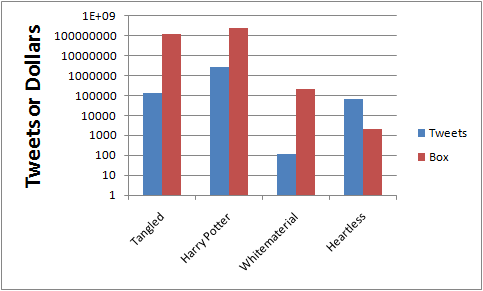
\includegraphics[scale=.5]{img/moviebox.png} 
\caption{Distribution of tweets by movie}
\end{figure}


\subsection{Stocks Analysis}
\begin{figure}[ht!]
\centering
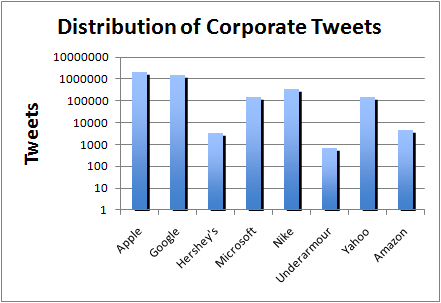
\includegraphics[scale=.65]{img/purestocktweets.png} 
\caption{Distribution of tweets by company}
\end{figure}

\section{Future Work}
In addition to the analyses we have already performed, there are many other methods that could be used in the future to further improve the accuracy and usefulness of this data.  For example, one such improvement that would be useful to implement in the future would be the implementation of a part of speech tagger for the tweet data.  Because the subjective word from �The Subjectivity Lexicon� list also includes a part of speech tag for each word, this method would allow us to categorize only the tweets whose subjective words match the part of speech of �The Subjectivity Lexicon�s� word.  For example, while the word �cool� is not in �The Subjectivity Lexicon,� but if it were, it would presumably only be included as a positive adjective (as in �that�s really cool�).  However, in the methods we used for this analysis, the noun form of cool (as in �it�s cool outside�) would also be counted as positive, even though this word is really more likely to be neutral, or possibly even negative.  In �The Subjectivity Lexicon,� this is also shown by the word �bullies�, which can be either a noun or verb.  According to the list, both words are negative, so this doesn�t affect the sentiment analysis much, but not all cases of homonyms work out so well.

Another improvement we could make in future analysis would be to implement a more effective negation algorithm.  While our negation algorithm is able to handle all cases of the form �not �subjective word��, this still leaves out many instances of negation, such as �not �non-subjective word� �subjective word�� or situations in which not is in the form of a conjunction, such as �don�t� or �can�t�.  However, implementing solutions to these problems without overcorrection (such as making the phrase �not just good, but great� negative when it is clearly positive) is very complicated, and so the best way to implement this would probably be to use a supervised algorithm such as the one proposed by Go et. al.   This supervised algorithm would also be useful for general, non-negated subjectivity as well, as it would allow us to identify other words that influence subjectivity that may not have been included in our initial list, which would result in a more accurate classification of the tweets.

Some of the problems in our data are simply due to difficulties in analyzing twitter data in general.  Because twitter does not allow users to search for any information before the most recent 1500 tweets, analysis can only be done on present tweets, so we were only able to gather data from November 16, 2010 to December 11, 2010.  While this works well for the movies we selected to analyze, as the movies were all released within this time frame, this does not allow us to compare our data to twitter data from past movie releases.  This was especially a problem for our situation, as the release of the highly anticipated seventh installment of Harry Potter certainly skewed our data, and also decreased the amount of competing movies available to analyze in depth (in fact,daily box-office reports of White Material and Heartless were unavailable because these movies did so poorly).  Because of this, our experiment would be much improved if it could be performed over a longer period of time, so different movies could be analyzed, as well as different weeks, which would allow for much more in-depth analysis of the relation between twitter and movie releases.  This would also be useful for the stock data, as our current analysis might not be the most accurate read of the relationship between twitter and stock performance simply due to the occurrence of Black Friday immeadiately preceding the period of our data collection, which might have some effect on sales. Essentially, due to our inability to poll past tweets, our data is constantly subject to the effect of current events, which frequently skews the data and interferes with potential correlation, and the only way to fix this is to gather information over a much longer period of time.

Another problem caused by our use of twitter is the fact that twitter users come from all over the world, while the box office data we used only comes from domestic data.  In fact, only 8\% of Americans use twitter, so our twitter data could be affected by foreign tweets, while our box-office data is purely domestic.  While this could be fixed slightly by only analyzing tweets in english, this solution would still include tweets from England and other english-speaking countries, which would still affect our data.  Overall, it seems the global quality of twitter will act as a limitation in most analyses of American situations, including movie releases, presidential popularity, and other events in which the comparison data is limited to the United States.
	
Overall, implementing all of the above strategies would almost certainly improve our sentiment analysis of twitter.  With these improvements, it would be very interesting to use our algorithm to further analyze the relationship  between twitter and various other objects subject to a range of sentiment and opinions.  This could include an analysis of people, such as the analysis of Obama and McCain presented in O�Connor et. al., as well as other political analyses, similar to the debate analysis presented by Diakopoulos and Shamma.  Twitter analysis could also be used to determine the popularity of specific places, such as amusement parks or museums, as well as the popularity of events.  Event analysis could even be used in comparing two events, such as John Stewart and Stephen Colbert�s Rally to Restore Sanity and/or Fear in comparison with Glenn Beck�s Restoring Honor Rally.  Furthermore, twitter analysis could be used to analyze to popularity of holidays, particularly less popular holidays such as labor day or veteran�s day.  Overall, the possibilities for twitter analysis are almost limitless, and are becoming more and more useful as twitter grows daily.

\section{Appendix}
\subsection{Synopses of included Movies}
The following brief synopses are taken from RottenTomatoes.com, a popular aggregator of movie reviews written by a diverse set of critics.

\textbf{Harry Potter and the Deathly Hallows-}In this seventh and final installment of the beloved Harry Potter series, Harry faces new troubles; he must collect all of the Horcruxes that the evil Lord Voldemort has left behind. He has no idea where these are and he has to destroy them all, even without the faintest idea how to do so.
 %rotten tomatoes
 
\textbf{Tangled-} Walt Disney Pictures presents "Tangled," one of the most hilarious, hair-raising tales ever told. When the kingdom's most wanted-and most charming-bandit Flynn Rider (voice of Zachary Levi) hides out in a mysterious tower, he's taken hostage by Rapunzel (voice of Mandy Moore), a beautiful and feisty tower-bound teen with 70 feet of magical, golden hair. Flynn's curious captor, who's looking for her ticket out of the tower where she's been locked away for years, strikes a deal with the handsome thief and the unlikely duo sets off on an action-packed escapade, complete with a super-cop horse, an over-protective chameleon and a gruff gang of pub thugs. In theaters this holiday season in Disney Digital 3D(TM), "Tangled" is a story of adventure, heart, humor and hair-lots of hair. -- (C) Disney

\textbf{Heartless-} Jim Sturgess (21, ACROSS THE UNIVERSE) leads a hugely-talented ensemble cast in this sublime British psychological thriller from cult UK director Philip Ridley (THE REFLECTING SKIN, THE PASSION OF DARKLY NOON), who returns to the screen after a 14-year absence. The film follows Jamie Morgan (Sturgess), born with a disfiguring birthmark across his face, which leaves him an outcast in rough East London. While wandering abandoned yards taking photographs, he comes across a gang of thugs and soon discovers that they are something other than human. He then is led into a Faustian deal that will see him become a party to the terrifying chaos around him. Part DONNIE DARKO, part Guillermo del Toro, this dark urban tale takes its audience to the darkest and most violent corners of the human heart. The film also stars Clémence Poésy, Noel Clarke, Joseph Mawle, Eddie Marsan, Luke Treadaway and Timothy Spall, and was produced by Pippa Cross and Richard Raymond. The film recently won the Best Independent Film Award at the Toronto After Dark Festival. --© IFC

\textbf{White Material-} From Claire Denis, the incomparable director of BEAU TRAVAIL, L'INTRUS and 35 SHOTS OF RHUM, comes WHITE MATERIAL: a rich and thrilling account of a woman driven to the edge. An official selection of the Venice, Toronto and New York Film Festivals, the film is a riveting exploration of the complexities of racial conflict and the limits of human will. The legendary Isabelle Huppert (LA CEREMONIE, THE PIANO TEACHER, 8 WOMEN), is Maria Vial, a fearless French woman attempting to run her family's coffee plantation in an unnamed African country. Torn violently apart by hate-fueled civil conflict, this unforgiving setting soon turns against the foreign family, declaring them outlaws in their new home. In a brash effort to save her family and livelihood, Maria risks everything, fighting with every shred of her will to buck the rebel forces wrestling for control of local power. --© IFC

%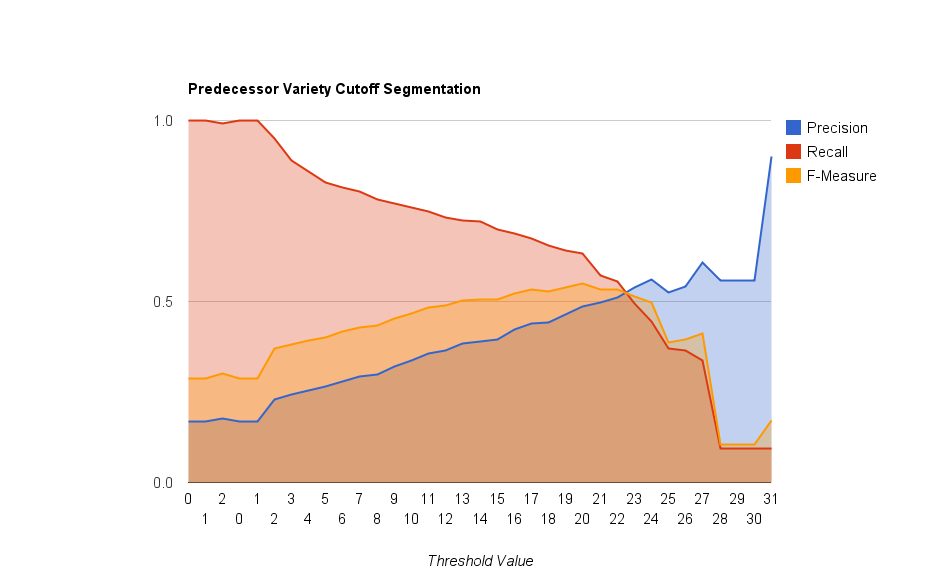
\includegraphics{img/PredVarietyChart.png}
%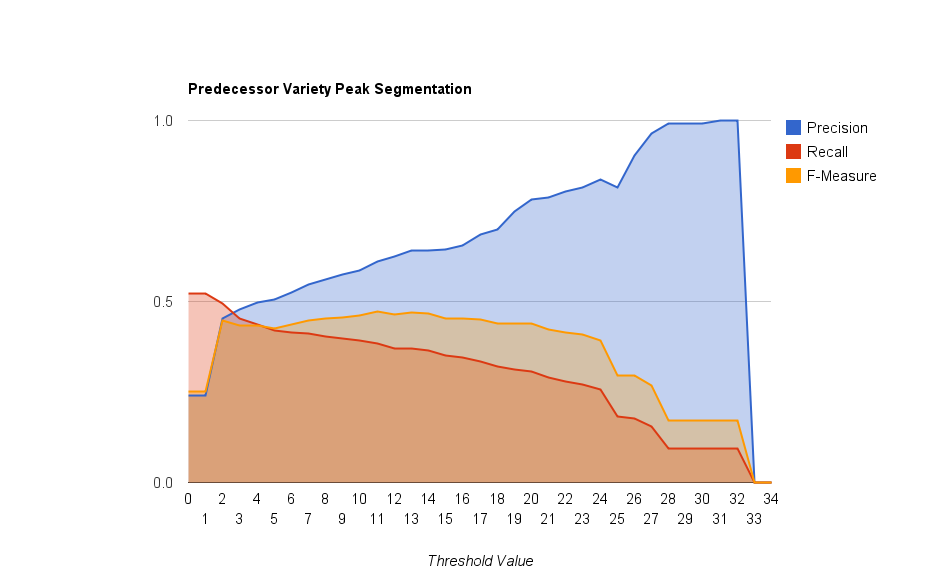
\includegraphics{img/PredVarPeak.png}
%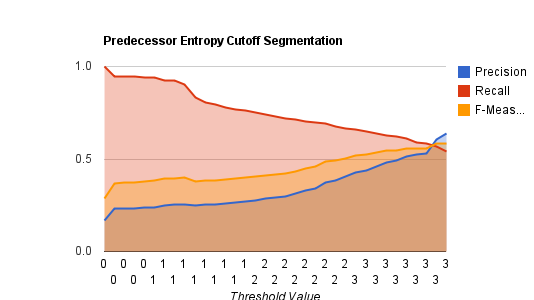
\includegraphics{img/PredEntCutoff.png}
%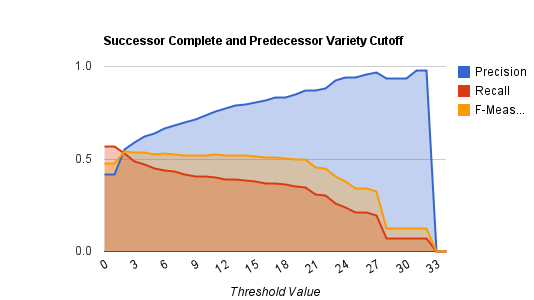
\includegraphics{img/SucCompandPredCut.png}
%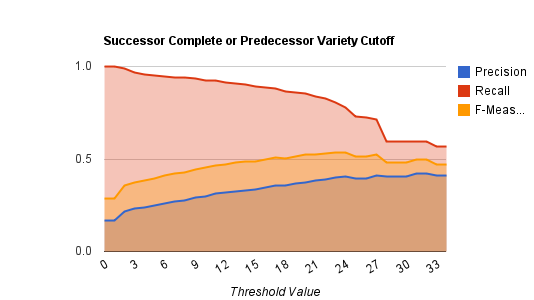
\includegraphics{img/SucComporPredCut.png}







\bibliographystyle{cs65f10}
\bibliography{cs65f10}

\end{document}
